
\section*{HS9: Főzőüst gömbfalának hővesztesége}
\addcontentsline{toc}{section}{Főzőüst gömbfalának hővesztesége}
\begin{tabular}{ | p{2cm} | p{14cm} | } 
	\hline
	Név: & Drávai Tamás László GHKELE\\ 
	\hline
	Szak: & Mechatronikai mérnök \\ 
	\hline
	Félév: & 2019/2020 II. (tavaszi) félév \\ 
	\hline
\end{tabular}
\vspace{4mm} 
%\\HS9 feladat:\\
\\Határozzuk meg egy gömb alakú főzőüst falán keresztül előálló hőveszteséget (W).  Ha az üst belső átmérője $\SI{1,2}{\meter}$  az üst falának és szigetelő rétegének együttes vastagsága $\SI{0,1}{m}$. A belső felület hőmérséklete $T_1=\SI{140}{\celsius}$ , a külső felület hőmérséklete  $T_2=\SI{140}{\celsius}$,  a hővezetési tényezője $\lambda=\SI[per-mode=fraction]{0,1396}{\watt\per\meter\per\kelvin}$.
\subsection*{ {Adatok:}}
\begin{equation*}
D_1=\SI{1,2}{\meter}  \quad  D_2=\SI{1,4}{\meter} \quad \delta=\SI{0,1}{\meter}\quad
\lambda=\SI[per-mode=fraction]{0,1396}{\watt\per\meter\per\kelvin}
\end{equation*}
\subsection*{Feladat megoldás:}
Alap összefüggés felírása:
\begin{equation}
\dot{Q}_{\textit{veszt}} =\pi \lambda\Delta T \dfrac{D_1 \cdot D_2}{\delta}
\end{equation}
\vspace{3mm}
Behelyettesítés a képletbe:
\begin{equation}
\dot{Q}_{\textit{veszt}}=\pi  \SI[per-mode=fraction]{0,1396}{\watt\per\meter\per\kelvin} \SI{90}{\kelvin}
\dfrac{\SI{1,2}{\meter} \cdot \SI{1,4}{\meter}}{\SI{0,1}{\meter}}
\end{equation}
Egyenlet rendezés és számítások elvégzése. 
\begin{equation}
\dot{Q}_{\textit{veszt}}=\SI{663,11}{\watt}
\end{equation}\\
A fözőüst falán keresztül fellépő hőveszteség az $\SI{663,11}{\watt}$.\\
\begin{figure}[h]
	\centering
	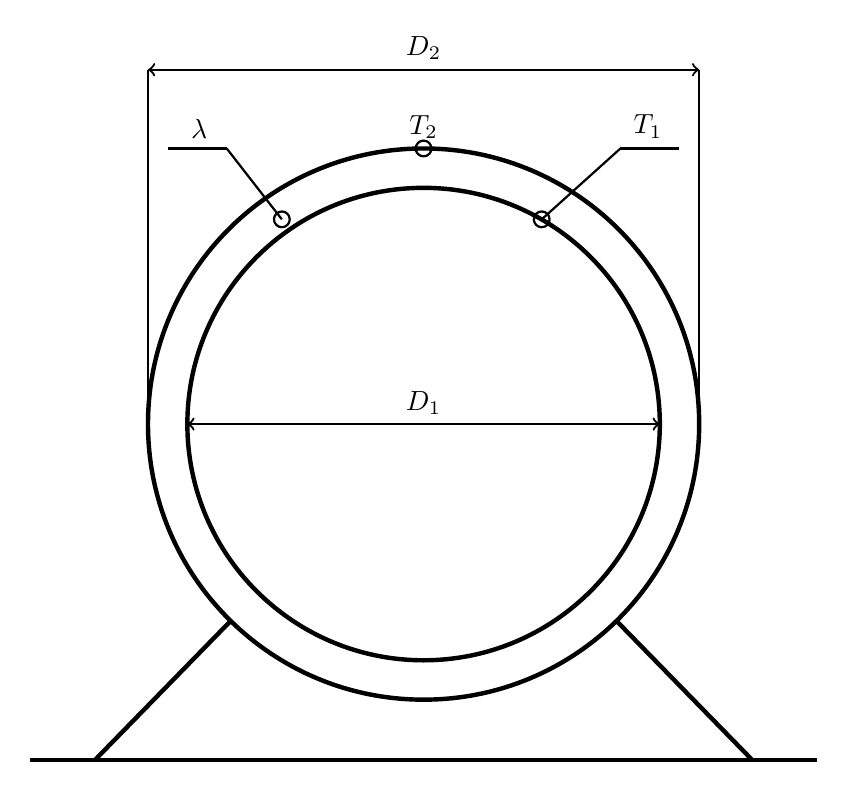
\begin{tikzpicture}
	%\draw[] (-6, -6) rectangle (6, 6); rajz keret
	\draw[color =black, ultra thick] (0, 0) circle (30 mm); %belső fal
	\draw[color =black,ultra thick] (0, 0) circle (3.5 ) ;%külső fal
	\draw[thick,<->] (-3,0) -- (3,0);% méretnyíl
	\draw (0,0)  node[above] { $\diameter D_1$};
	\draw[thick,<->] (-3.5,4.5) -- (3.5,4.5); %felső méretnyíl
	\draw (0,4.5)  node[above] {$\diameter D_2  $};
	\draw [thick] (-3.5,0) -- (-3.5,4.5) (3.5,0) -- (3.5,4.5); %%felső méretnyíl oldalt
	\draw [ultra thick] (-2.45,-2.5) -- (-4.175,-4.2675) (2.45,-2.5) -- (4.175,-4.2675); %lábak
	\draw [ultra thick] (-5,-4.2675) -- (5,-4.2675) ;%földvonal		
	fill[pattern={Lines[angle=45, distance=2mm]}] (-5, 0) rectangle (5, -0.5);%földvonalak
	%T1
	\draw [thick] (1.5,2.6) circle (0.1) (1.5,2.6) -- (2.5,3.5)  ;
	\draw [thick]  (2.5,3.5) -- (3.25,3.5) ;
	\draw [thick](2.85,3.5)  node[above] {$T_1$};
	% lambda
	\draw [thick] (-1.8,2.6) circle (-0.1) (-1.8,2.6) -- (-2.5,3.5)  ;
	\draw [thick]  (-2.5,3.5) -- (-3.25,3.5) ;
	\draw (-2.85,3.5)  node[above] {$\lambda$};
	%T2
	\draw [thick] (0,3.5) circle (0.1) ;
	\draw (0,3.5)  node[above] {$T_2$};
	
	\end{tikzpicture}
	\caption{Gömb alakú főzőüst}
\end{figure}

\begin{figure}
	%\centering
	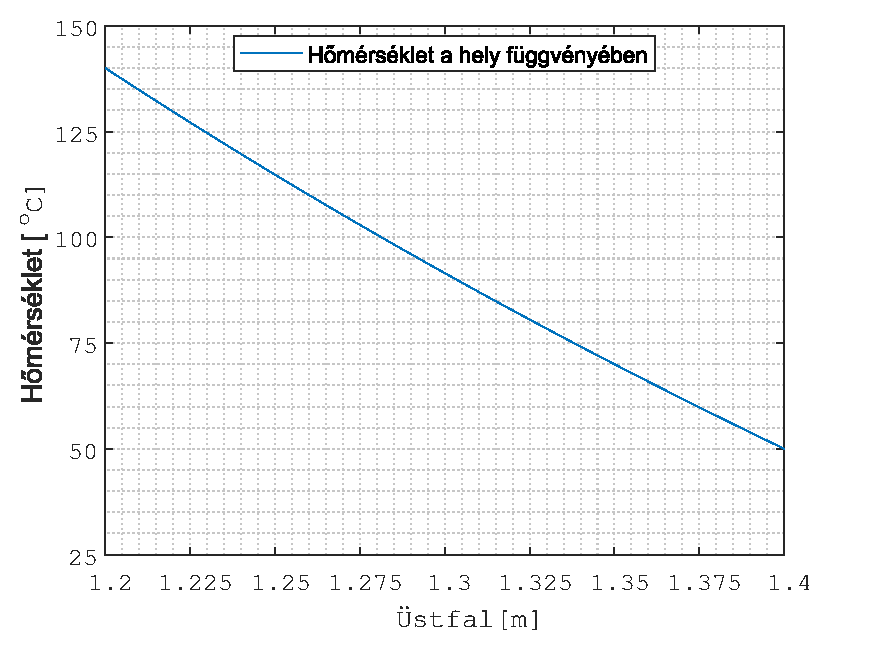
\includegraphics[width=1\linewidth]{homersekletfuggvenyHS9.eps}
	\caption{}
	\label{fig:waveforms}
\end{figure}

\end{document}